\documentclass[a4paper,titlepage]{article}
\usepackage{ascmac}
\usepackage{amsmath,amssymb}
\usepackage{siunitx}
\sisetup{group-separator = {,}}
\usepackage[dvipdfmx]{graphicx}

\usepackage{listings}
\usepackage{color}

\lstset{
language={Ruby},
basicstyle={\small\ttfamily},
identifierstyle={\small},
commentstyle={\small\ttfamily \color[rgb]{0,0.5,0}},
keywordstyle={\small\ttfamily\bfseries \color[rgb]{1,0,0}},
ndkeywordstyle={\small},
stringstyle={\small\ttfamily \color[rgb]{0,0,1}},
frame={tb},
breaklines=true,
columns=[l]{fullflexible},
numbers=left,
xrightmargin=0zw,
xleftmargin=3zw,
numberstyle={\scriptsize},
stepnumber=1,
numbersep=1zw,
morecomment=[l]{//}
}

\newcommand{\Cost}{\mathrm{Cost}}
\newcommand{\Price}{\mathrm{Price}}
\newcommand{\Power}{\mathrm{Power}}
\newcommand{\toluene}{\mathrm{toluene}}
\newcommand{\coolant}{\mathrm{coolant}}
\newcommand{\steam}{\mathrm{steam}}
\newcommand{\reactor}{\mathrm{reactor}}

\begin{document}
  \title{Process System Engineering \#5}
  \author{\#03150796 Amane Suzuki}
  \date{November 4, 2015}
  \maketitle

  \section{Abstract}
  We use the Steepest Descent Method to find the minimum of functions.
  Steepest Descent Method can calculate the minimum of simple funcion enough fast and accurate.
  However when find the minimum of little complicated function, processing time is much longer depending on initial condition.

  \section{Algorithm}
  We use Steepest Descent Method to find the minimum of following two functions.
  \begin{align}
    f(x,y) &= (x-1)^2 + 50(y-1)^2 \\
    g(x,y) &= (x-1)^2 + 100(x^3-y)^2
  \end{align}

  Figure \ref{fig:sdm} shows a flow of Steepest Descent Method.

  \begin{figure}[htbp]
    \centering
    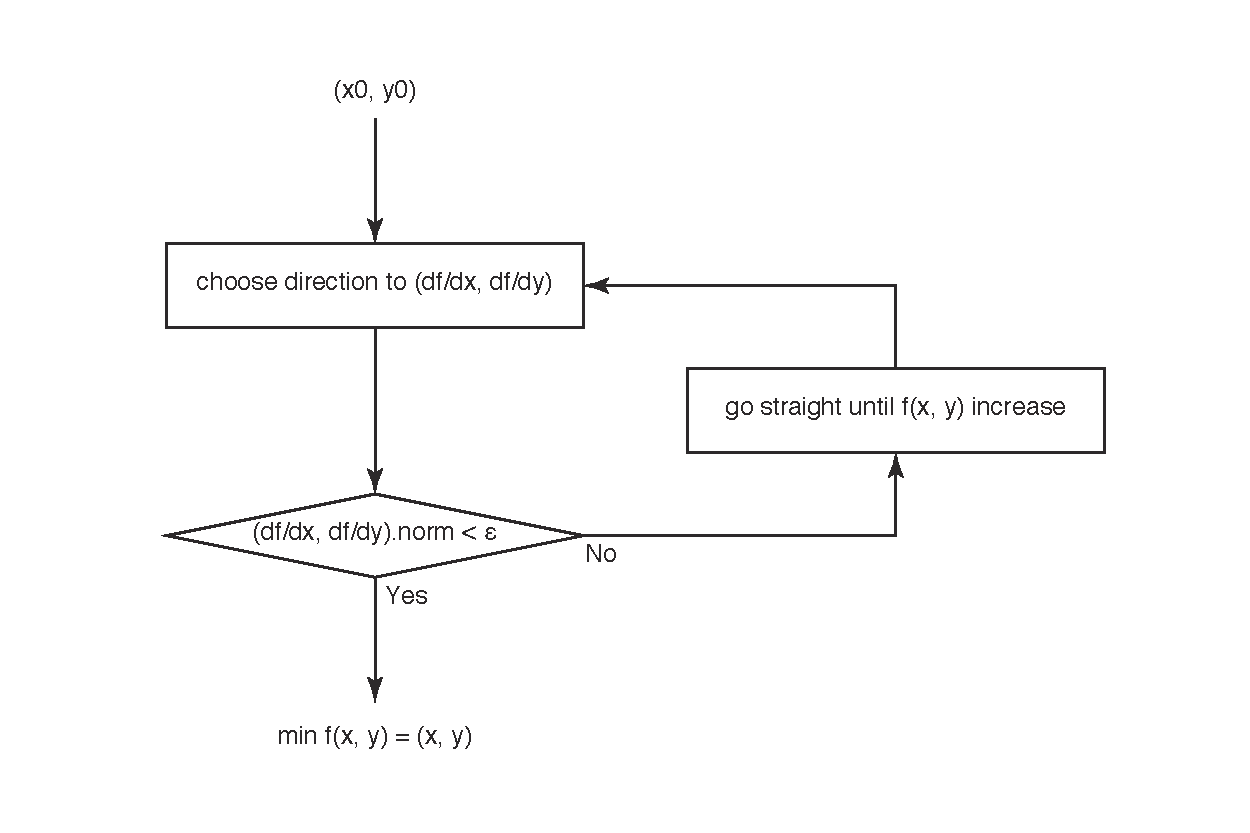
\includegraphics[width=12cm]{images/sdm.pdf}
    \caption{The flow chart of steepest decent method.}
    \label{fig:sdm}
  \end{figure}

  First, this method choose direction where function decreases steepest.
  \begin{align}
    (\mathrm{direction vector}) = - \left(\frac{\partial f}{\partial x} , \frac{\partial f}{\partial y}\right)
  \end{align}

  If the direction vector is sufficiantly small, this method regard $(x,y)$ of that time as the minimum of the funcion.
  After decided direction vector, it try going straight until the function increases.
  Repeating these operations, $(x,y)$ approach to the minimum.

  Steepest Descent Method is easy to coding because it only uses first derivation. It has, however, a few demerits.
  \begin{itemize}
    \item Depending on the initial $(x,y)$, it approach to \emph{local} minimum.
    \item Steepest Descent does NOT mean fastest method to find minimum.
    \item It needs partial differential of the funcion.
  \end{itemize}

  \section{Result}
  \subsection{Find minimum of $f(x,y)$ with $(x_0, y_0)=(0,0)$}
  \begin{verbatim}
$ ruby optimize.rb
Vector[0.9999999999998566, 1.0000000000000009]
0.015027 sec\end{verbatim}

  Numerical solution is $(x,y) = (0.9999999999998566, 1.0000000000000009)$. It means this method can find the correct minimum of $f(x,y)$.
  (cf. Analytical solution is $(x,y)=(1,1)$)

  \subsection{Benchmark of finding $min(f(x,y))$}

  Table \ref{tb:benchmark-f} shows the result of benchmark.
  In this benchmark, we choose 10000 initial condition at random, test whether it approach the true minimum, and measure the processing time.

  Pass means the result is correct. Fail means the result is wrong. Timeout means processing time is over 3 second.
  Average Time is the agerage time of \emph{Pass} cases.

  \begin{table}[htbp]
    \centering
    \begin{tabular}{ll}\\\hline
      Pass & 10000 \\\hline
      Fail & 0 \\\hline
      Timeout & 0 \\\hline
      Average Time & 0.023 sec \\\hline
    \end{tabular}
    \caption {Benchmark of finding minimum of $f(x,y)$}
    \label{tb:benchmark-f}
  \end{table}

  The result shows that this method is useful finding the minimum of function $f$.

  \subsection{Find minimum of $g(x,y)$ with $(x_0, y_0)=(0,0)$}
  \begin{verbatim}
$ ruby optimize.rb
Vector[0.9984717014948186, 0.9954053544707571]
1.33843 sec\end{verbatim}

  Numerical solution is $(x,y) = (0.9984717014948186, 0.9954053544707571)$. It means this method can find the correct minimum of $g(x,y)$.
  (cf. Analytical solution is $(x,y)=(1,1)$)

  \subsection{Benchmark of finding $min(g(x,y))$}
  Table \ref{tb:benchmark-g} shows the result of benchmark.

  \begin{table}[htbp]
    \centering
    \begin{tabular}{ll}\\\hline
      Pass & 7663 \\\hline
      Fail & 0 \\\hline
      Timeout & 2337 \\\hline
      Average Time & 1.04 sec \\\hline
    \end{tabular}
    \caption {Benchmark of finding minimum of $g(x,y)$}
    \label{tb:benchmark-g}
  \end{table}

  When finding the minimum of function $f$, this method has enough speed and accuracy. In contrast,
  when finding the minimum of function $g$, there is 2337 timeouts.

  Figure \ref{fig:timeouts} shows the plot of initial conditions that goes timeout.

  \begin{figure}[htbp]
    \centering
    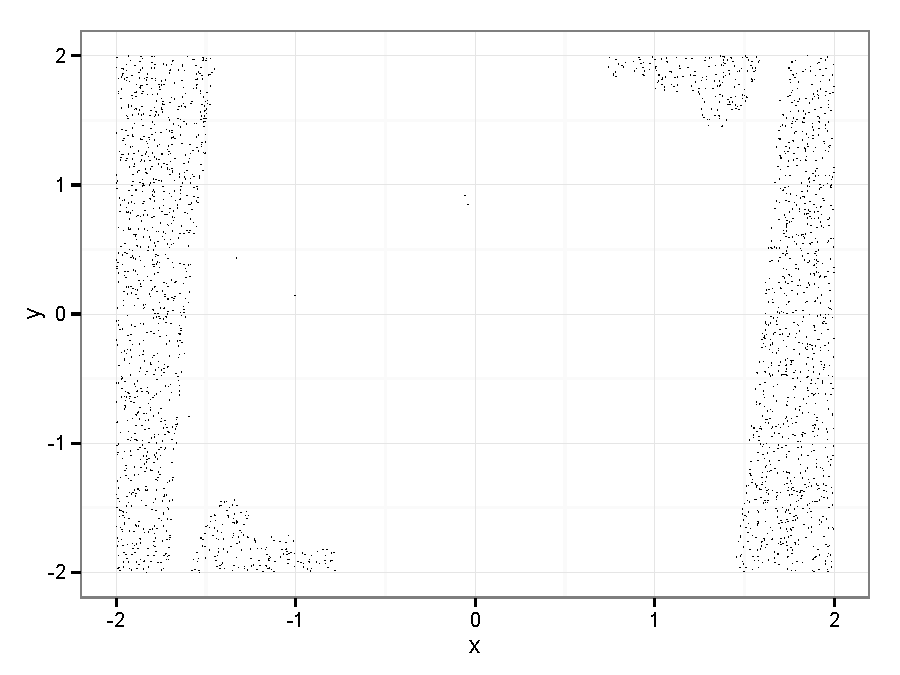
\includegraphics[width=12cm]{images/timeouts.pdf}
    \caption{The initial conditions of Timeout cases.}
    \label{fig:timeouts}
  \end{figure}

  \section{Discussion}
  Steepest Descent Method can calculate the minimum of simple funcion enough fast and accurate.
  Using to a function which has deep valley (e.g. $g(x,y)$), we have to choose initial condition carefully or execute a lot of trials.

  Proper initial condition doesn't mean coordinate which is near solution and isn't easy to find,
  therefore we should calculate in a variety of initial conditions.

  \section{Source Program}
  \lstinputlisting[caption=optimize.rb, label=code:optimize]{code/optimize.rb}
\end{document}
